\begin{frame}
\frametitle{Context-dependent Non-word Correction Data}
\begin{itemize}
    \item 1,686 3-4 character words from Aspell English dictionary with 100+ occurrences in English Wikipedia
    \item Sampled 100-1000 contexts for each word ({\textasciitilde}1.5m)
    \item Context = window of width 5 centered on word 
    \item Eliminated duplicate and OOV contexts ({\textasciitilde}935k remained)
    \item {\textasciitilde}850k train, {\textasciitilde}5k validation, {\textasciitilde}80k test 
\end{itemize}
\end{frame}

\begin{frame}
\frametitle{Context-dependent Non-word Correction Models}
\begin{itemize}
    \item 1-4 Gram language model 
        \begin{itemize}
            \item Google Web 1T 5-gram Version 1 
            \item Good-Turing discounting
            \item Backoff
        \end{itemize}
    \item Feed-forward Embedding Network (Word only)
        \begin{itemize}
            \item Window of 5 words centered on non-word
            \item 200-dimensional word embeddings (= 1000-dimensional input to residual block)
        \end{itemize}
    \item ConvNets (Word only, Word and Character)
        \begin{itemize}
            \item 1000 filters of width 5 for width-5 word inputs
            \item 100 filters of width 3 for non-word and candidate character inputs
            \item Word ConvNet = 1000-dimensional input to residual block)
            \item Word and Character ConvNet = 1200-dimensional input to residual block
        \end{itemize}
\end{itemize}
\end{frame}

\begin{frame}
\frametitle{Feed-forward Embedding Block}
\centering
\begin{figure}
\input figures/chapter05/feedforward-embedding.tex
\end{figure}
\end{frame}

\begin{frame}
\frametitle{Word Convolutional Block Input}
\centering
\begin{figure}
\input figures/chapter05/convnet-word.tex
\end{figure}
\end{frame}

\begin{frame}
\frametitle{Character Convolutional Block Input}
\centering
\begin{figure}
\input figures/chapter05/convnet-character.tex
\end{figure}
\end{frame}

\begin{frame}
\frametitle{Residual Block}
All networks have a stack consisting of 1 fully-connected layer and 4 residual blocks before softmax output layer. 
\centering
\begin{figure}
\input figures/chapter05/residual-block.tex
\end{figure}
\end{frame}

\begin{frame}
\begin{figure}
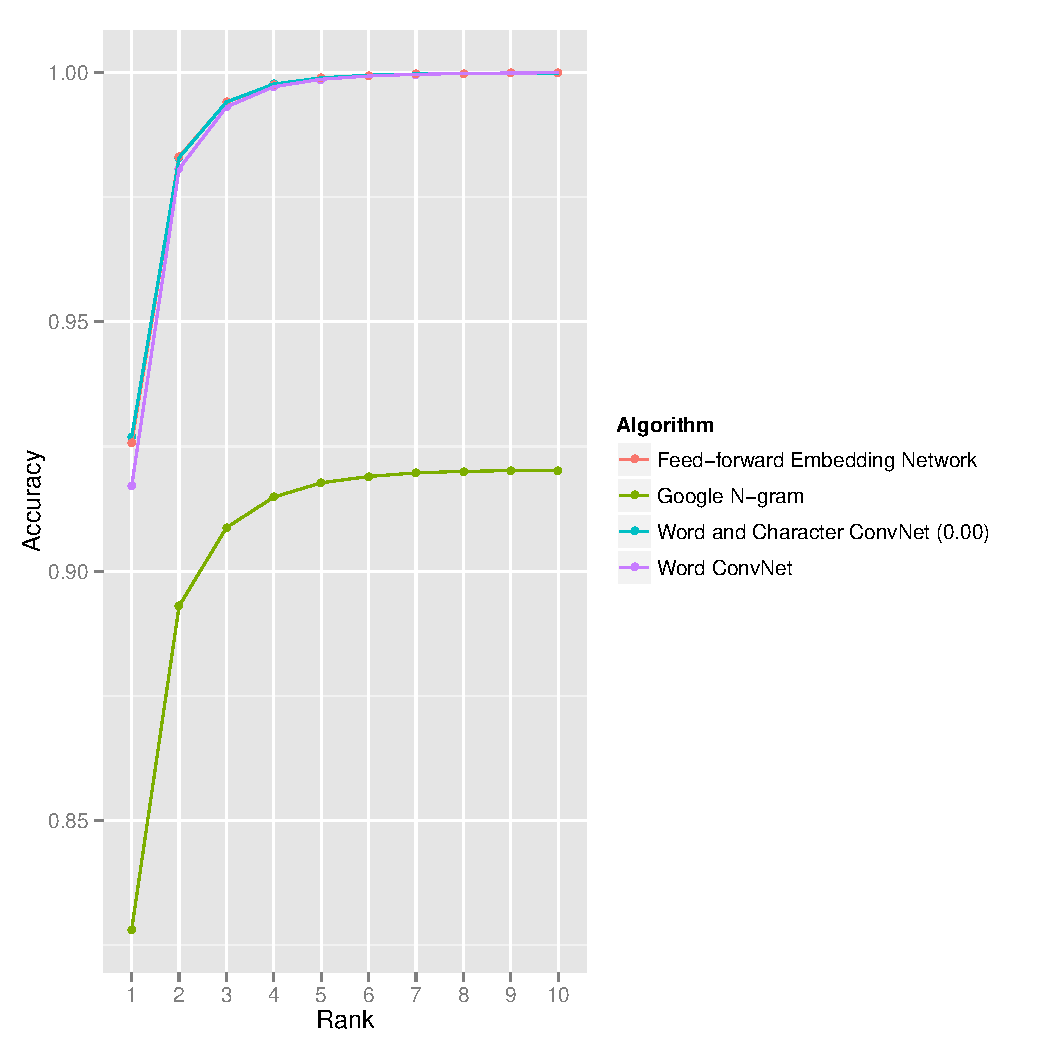
\includegraphics[height=\textheight]{figures/chapter05/accuracy-at-k-binary-contextual}
\end{figure}
\end{frame}

\begin{frame}
\input figures/chapter05/comparison-of-convnet-and-google.tex
\end{frame}

\begin{frame}
\centering
\begin{table}[]
\begin{tabular}{lrrrr}
\hline
%\textsc{RANK Model} & \textsc{Spearman's} $\rho$ & \textsc{Kendall's} $\tau$ \\
\textsc{RANK Model} & \textsc{Kendall's} $\tau$ \\
\hline
%Google Web 1T 5-gram Corpus & -0.19 & -0.14 \\
Google Web 1T 5-gram Corpus & -0.14 \\
%Feed-forward Embedding Net & -0.04 &  -0.03 \\
Feed-forward Embedding Net & -0.03 \\
%ConvNet (Word) & -0.04 &  -0.03 \\
ConvNet (Word) & -0.03 \\
%ConvNet (Word and Character) & -0.04 & -0.03 \\
ConvNet (Word and Character) & -0.03 \\
\hline
\end{tabular}
\caption{Rank correlation of a model's rankings and the unigram probability of the candidate.} 
\end{table}
\end{frame}

\begin{frame}
\centering
\begin{table}

\begin{tabular}{c|cccc}
           & \multicolumn{4}{c}{\textsc{RANK}} \\
           \hline
$\sigma^2$ & 1 & 2 & 3 & 4 \\
\hline
.00        & .927 & .983 & .994 & .998 \\
.01        & .929 & .984 & .994 & .998 \\
.02        & .951 & .989 & \textbf{.997} & \textbf{.999} \\
.03        & .952 & .990 & .996 & .999 \\
.04        & .951 & .989 & .996 & .999 \\
.05        & .947 & .988 & .996 & .998 \\
.06        & \textbf{.954} & \textbf{.991} & \textbf{.997} & \textbf{.999} \\
.07        & .940 & .986 & .995 & .998 \\
.08        & .941 & .987 & .995 & .998 \\
.09        & .930 & .984 & .994 & .998 \\
.10        & .951 & .990 & \textbf{.997} & \textbf{.999} \\
\end{tabular}
\caption{Effect of varying the noise $\mathcal{N}(0, \sigma^2)$ with which the Word and Character ConvNet was trained.}
\end{table}
\end{frame}